%% ****** Start of file apstemplate.tex ****** %
\documentclass[aps,prl,reprint,groupedaddress]{revtex4-2}

% You should use BibTeX and apsrev.bst for references
% Choosing a journal automatically selects the correct APS
% BibTeX style file (bst file), so only uncomment the line
% below if necessary.
% \bibliographystyle{apsrev4-2}

\usepackage{graphicx}
\usepackage{epstopdf}
\usepackage{amsmath}
\usepackage{amsthm}
\usepackage{amsfonts}
\usepackage{subfigure}
\usepackage{hhline}
\usepackage[left=1cm,right=1cm,top=1cm,bottom=1cm]{geometry}
\usepackage[miktex]{gnuplottex}
\usepackage{xcolor}
\usepackage{amssymb}
\usepackage{amsmath}
\usepackage{color}
\usepackage{hyperref}
\usepackage[percent]{overpic}
\usepackage{tikz}
\usepackage{mathrsfs}
\usepackage{wasysym}
\usepackage{tikz-cd}
\usepackage{caption}  % Elimina hypcap=true si está presente
\usepackage{stackengine,scalerel}

\usepackage{caption}
\captionsetup{skip=0pt}  % Reduce el espacio entre la imagen y su caption
\raggedbottom

% so sections, subsections, etc. become numerated.
\setcounter{secnumdepth}{3}

\newenvironment{Figura}
  {\par\medskip\noindent\minipage{\linewidth}}
  {\endminipage\par\medskip}

\renewcommand{\appendixname}{Apéndice} % Change "Appendix" to "Apéndice"

\begin{document}

%Title of paper
\title{
Fashion-MNIST con PyTorch
}

% autores
\author{Kevin Gaston Mansilla}
\email[]{kevin.mansilla@mi.unc.edu.ar}

\affiliation{}

%fecha
\date{\today}

\begin{abstract}
En este trabajo se implementa una red feed forward autoencoder para clasificar
imágenes de Fashion-MNIST. Se entrenan tres modelos con diferentes hiperparámetros
y se comparan los resultados obtenidos por medio de la precisión y la 
pérdida (loss). Se observa que el modelo 2, que utiliza el optimizador Adam, 
tiene un mejor desempeño que el modelo que usa un optimizador SGD, ya que
converge más rápido y tiene una precisión más alta. Por otro lado, se observa que
aumentar las épocas de entrenamiento no necesariamente mejora el desempeño de la
red, ya que el modelo 3, que tiene el doble de épocas que el modelo 2, tiene una
precisión similar.
\end{abstract}

% insert suggested keywords - APS authors don't need to do this
%\keywords{}

%\maketitle must follow title, authors, abstract, and keywords
\maketitle

\section{Introducción}
Las redes feed forward son un tipo de red neuronal que están compuestas por 
$N$ capas donde $N-1$ son capas ocultas. La primera capa no se contabiliza 
porque es la capa de entrada. La particularidad de estas redes es que las 
conexiones se realizan entre capas consecutivas, es decir, no hay conexiones
entre capas no consecutivas, como lo muestra la Figura \ref{fig-feed-forward}.
\begin{Figura}
  \centering
  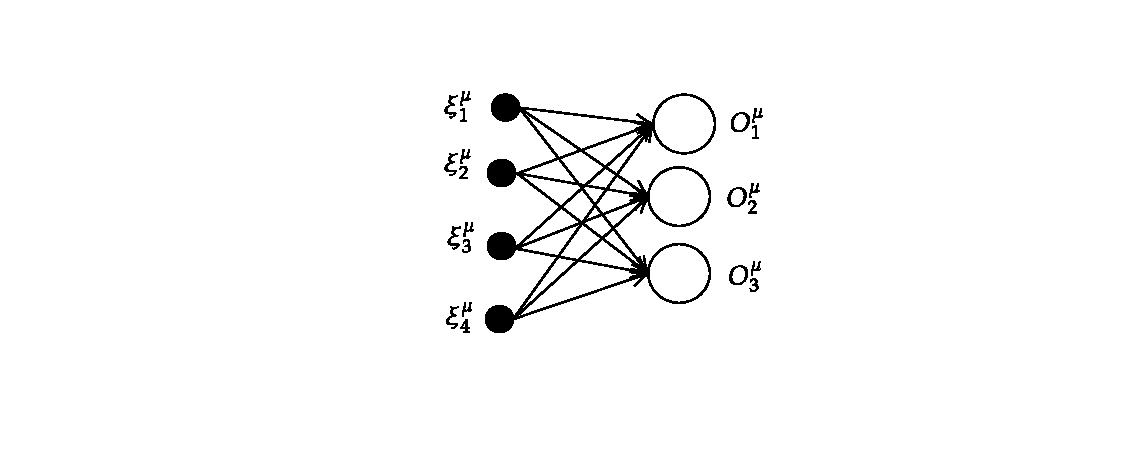
\includegraphics[width=1\textwidth]{figs/red-feed-forward.pdf}
  \captionof{figure}{Red feed forward}
  \label{fig-feed-forward}
\end{Figura}

Puede computarse la salida de la red mediante la siguiente ecuación:
\begin{equation}
  O^{\mu}_{i} = g(h_{i}) - g \left( \sum_{k} w_{ik} \xi_{k} \right)
  \label{eq-feed-forward}
\end{equation}

En la ecuación \ref{eq-feed-forward}, da información de la relación o conexión 
entre las neuronas de entrada ($\xi_{k}$) y las neuronas de salida 
($O^{\mu}_{i}$) se representa por medio de los ponderadores $w_{ik}$, 
donde $i$ es el índice de la neurona de salida y $k$ es el índice de la 
neurona de entrada. El cálculo de la salida dependerá de la función de 
activación $g$ y de la función de propagación $h_{i}$.

Al utilizar una red feed forward autoencoder, se busca que la red aprenda a
reconstruir la entrada en la salida, es decir, que la salida sea igual a la 
entrada. Por lo tanto, la red debe aprender a comprimir la información de 
entrada en una representación más pequeña, para luego descomprimir la 
información y obtener la salida. La red que usaremos será como 
\ref{fig-feed-forward-autoencoder}, donde $V_{j}$ es la función de activación 
de la capa oculta.

\begin{Figura}
  \centering
  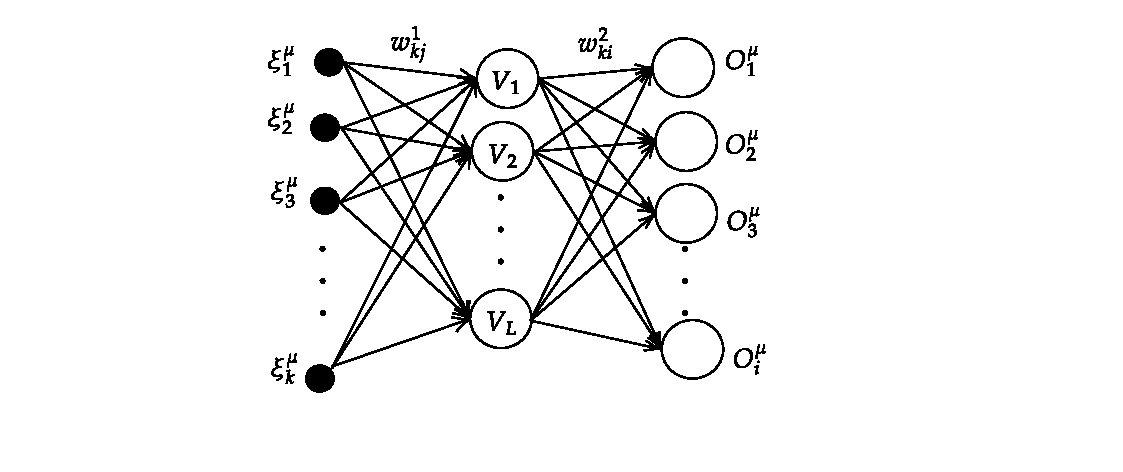
\includegraphics[width=1\textwidth]{figs/red-autoencoder.pdf}
  \captionof{figure}{Red feed forward autoencoder}
  \label{fig-feed-forward-autoencoder}
\end{Figura}

Este tipo de redes, tiene la particularidad de que la capa de entrada y la capa 
de salida deben tener la misma cantidad de neuronas, mientras que las capas 
intermedias deben tener una cantidad menor de neuronas. Esto obliga a la red a 
encontrar patrones entre los elementos de entrada y salida, de forma que aprenda 
a presentar la información comprimida y permitiendo así reducir la dimensionalidad 
de los datos. 

\section{Arquitectura de Red Neuronal}
En este trabajo, se implementará una red feed forward autoencoder al corpus 
Fashion-MNIST\footnote{https://github.com/zalandoresearch/fashion-mnist}, la 
cual consiste en un conjunto de imágenes de ropa en escala de grises de 
$28\times 28$ píxeles, conformadas por las siguientes categorias:
\begin{verbatim}
0: 'T-shirt/top',
1: 'Trouser',
2: 'Pullover',
3: 'Dress',
4: 'Coat',
5: 'Sandal',
6: 'Shirt',
7: 'Sneaker',
8: 'Bag',
9: 'Ankle boot'
\end{verbatim}

En la figura \ref{fig-sample} se muestran ejemplos de algunas categorias.
\begin{Figura}
  \centering
  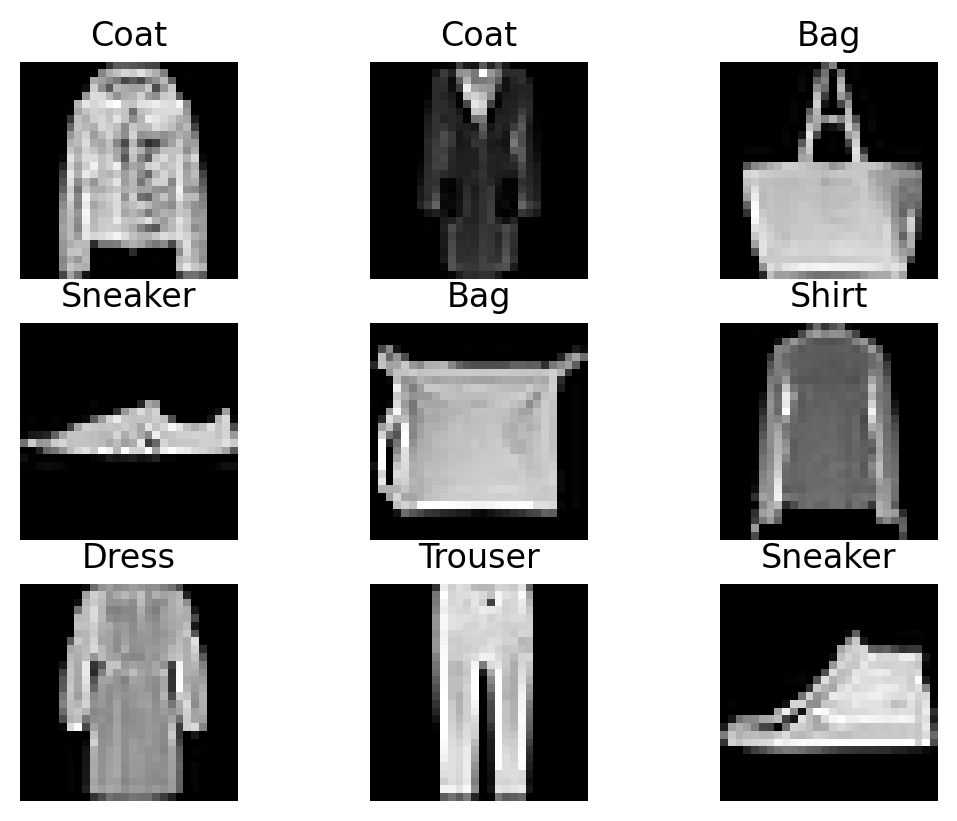
\includegraphics[width=1\textwidth]{figs/sample.png}
  \captionof{figure}{Arquitectura de la red neuronal\footnote{https://bea.stollnitz.com/blog/fashion-pytorch/}}
  \label{fig-sample}
\end{Figura}

Donde el principal objetivo es clasificar una imagen de entrada en una de las 
$10$ categorías. En la figura \ref{fig-red} se muestra la arquitectura de la red.
Donde se observa que a la imagen inicial en la capa $1$ se la aplica un 
\textit{flatten} para transformar la imagen de $28x28$ en un vector de $784$ 
elementos, luego pasa por la primera capa oculta de $n1$ neuronas la cual al 
inicio se le aplica un módulo \textit{lineal}, luego una función de activación 
\textit{ReLU} y finalmente se le aplica un módulo \textit{dropout} con una 
probabilidad de $0.2$.

Luego, la salida de la primera capa oculta pasa por la segunda capa oculta de $n2$
neuronas que tiene el mismo comportamiento que la capa anterior. Finalmente,
el flujo de la red llega a la capa final que tiene $10$ neuronas cada una 
representando una de las categorías de Fashion-MNIST. Asi el output final es un 
vector de $10$. En este ejemplo particular se puede ver que como input se paso 
una imagen de Ankle boot y como en el output final, el valor más alto se da en 
la posición $9$ significa que la red clasificó correctamente la imagen.

\begin{Figura}
  \centering
  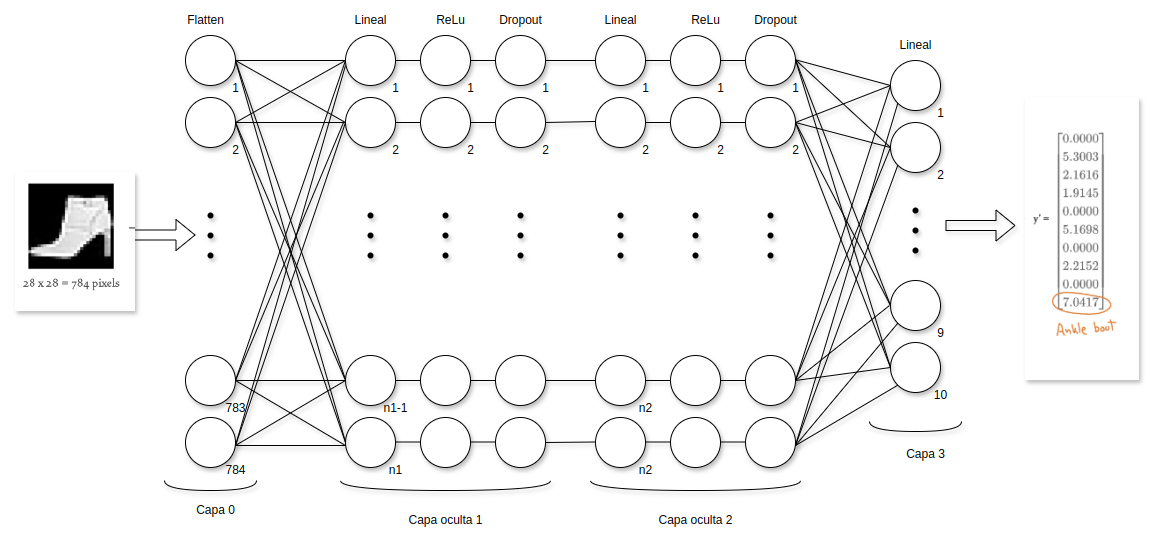
\includegraphics[width=1\textwidth]{figs/arq_model.png}
  \captionof{figure}{Arquitectura de la red neuronal}
  \label{fig-red}
\end{Figura}

Entonces se buscará entrenar esta red usando PyTorch, como función de perdida 
se utiliza el error cuadrático medio y el método de descenso 
por el gradiente estocástico como algoritmo de optimización (minimización), 
con un learning rate de $1e-3$ que indica 'de qué tamaño' dar el paso 
para que el algoritmo converja a la solución. Lo ideal es hacerlo de forma 
proporcional al gradiente, es decir, si el gradiente es grande, el paso será
grande y si el gradiente es pequeño, el paso será pequeño.

El proceso de descenso por el gradiente estocástico se realiza en mini-batches,
es decir, se toma un subconjunto de los datos de entrenamiento y se calcula el
gradiente para ese subconjunto. Luego se actualizan los pesos de la red y se
toma otro subconjunto de datos y se repite el proceso. Esto se hace para evitar
que la red se sobre ajuste a los datos de entrenamiento y no pueda generalizar
a datos nuevos.

Como base se utilizarán los siguientes hiperparámetros: $n1=128$, $n2=64$, 
$30$ épocas y un batch size de $100$ con un optimizador 
Stoachastic Gradient Descent (SGD) con un learning rate de $1e-3$. Luego se 
realizarán pruebas variando los hiperparámetros para ver cómo afectan al 
desempeño de la red. En particular, se cambiará el optimizador por Adam y 
por último se pasará a $60$ épocas, en la siguiente sección presentaremos
estos resultados

\section{Resultados}

Aquí presentaremos los resultados obtenidos al entrenar la red neuronal en los 
diferentes modelos planteados. Los hiperparámetros son:

\begin{itemize}
  \item Modelo 1 (Base): $n1=128$, $n2=64$, $30$ épocas y un batch size de $100$ 
  con un optimizador Stoachastic Gradient Descent (SGD) con un learning rate 
  de $1e-3$.
  \item Modelo 2: $n1=128$, $n2=64$, $30$ épocas y un batch size de $100$ con un
  optimizador Adam con un learning rate de $1e-3$.
  \item Modelo 3: $n1=128$, $n2=64$, $60$ épocas y un batch size de $100$ con un
  optimizador Adam con un learning rate de $1e-3$.
\end{itemize}

En la tabla \ref{tab:models} se presentan los resultados obtenidos para cada
modelo. Donde se puede observar que el modelo 2 y 3 tienen un mejor desempeño
que el modelo 1. Esto se debe a que el optimizador Adam es más eficiente que el
SGD, ya que este último no tiene en cuenta la dirección del gradiente, sino que
se mueve en la dirección opuesta al gradiente. Por otro lado, se observa que
el modelo 2 y el 3 tienen un desempeño similar, lo que significa que aumentar 
las épocas de entrenamiento no necesariamente mejora el desempeño de la red, 
en muchos casos puede producir overfitting.

Entonces, se puede concluir que el modelo 2 es el mejor modelo, ya que tiene un
mejor desempeño y menor tiempo de entrenamiento que el modelo 3.

\begin{table}[h!]
  \begin{tabular}{lccll}
    \hline
    Modelos         & Loss      & Presición & \\ \hline
    Modelo 1 (Base) & $0.51\% $ & $81.0\%$  & \\
    Modelo 2        & $0.32\% $ & $89.3\%$  & \\
    Modelo 3        & $0.37\% $ & $89.1\%$  & \\ \hline
  \end{tabular}
  \caption{Resultados del entrenamoento de la red neuronal}
  \label{tab:models}
\end{table}

En la figura \ref{fig-ap12} se muestran las curvas de precisión y loss para los
modelos 1 y 2. En la parte $a)$ se observa que con SGD la pérdida inicial es 
considerablemente más alta que la de Adam, lo cual indica que converge más 
lentamente. A su vez, a medida que aumentan las épocas, la pérdida se reduce 
gradualmente, pero nunca alcanza los valores de Adam, lo que indica que este 
optimizador es más eficiente que el SGD. En ambos modelos, la brecha 
entre la curva de entrenamiento y validación es pequeña, lo que indica que no
hay sobreajuste.

Por otra parte, en la parte $b)$ Adam logra una alta precisión mucho más rápida
que SGD. Aunque este último mejora constantemente, no alcanza los valores de Adam. 
Una observación importante es que en Adam las curvas de entrenamiento y 
valuación son casi idénticas lo cual demuestra que el modelo es robusto y 
generaliza bien.

Entonces se puede decir que Adam tiene un desempeño superior tanto en términos 
de reducción de pérdida como en precisión, mostrando una convergencia más 
rápida y resultados más estables. Y SGD es más lento en converger y menos
estable en términos de precisión. 

\begin{Figura}
  \centering
  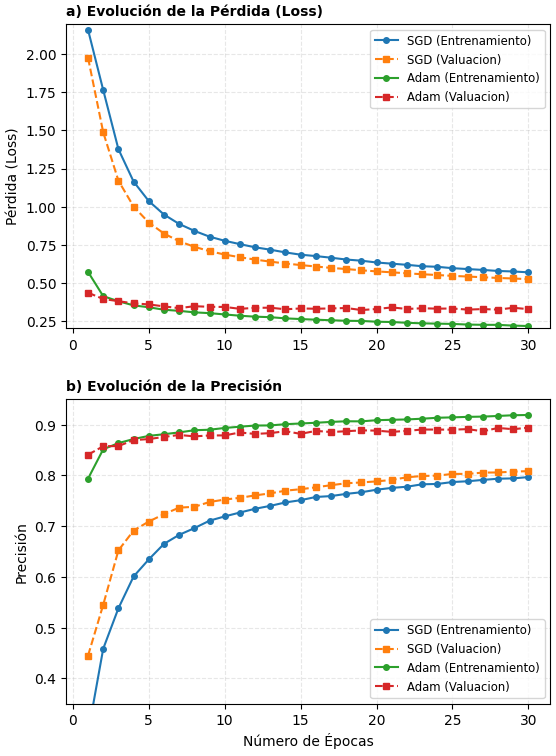
\includegraphics[width=1\textwidth]{figs/modelos_plots.png}
  \captionof{figure}{Presición y Loss de los modelos 1 y 2}
  \label{fig-ap12}
\end{Figura}

Como se mencionó anteriormente, el modelo 2 es el mejor modelo, por lo que 
resulta interesante analizar la matriz de confusión. En la figura \ref{fig-matriz2}
los elementos de la diagonal principal se corresponden con los elementos 
correctamente clasificados, y se observa que son bastante altos en la mayoria de 
los casos. Mientras que los elementos por fuera de la diagonal principal son 
elementos que la red clasifica incorrectamente, por ejemplo, la red clasifica 
T-shirt/top como Shirt en $75$ casos, lo cual es un error común, ya que ambas 
categorías son similares.

Por otra parte, en Shirt el error es mayor, en la gran mayoría de los casos 
se clasifica como T-shirt/top, Coat, Pullover y en menor medida
como Dress. Esto se debe a la similitud entre las categorías, ya que todas
son prendas de vestir superiores. Por otro lado, en Sneaker el error es menor, 
ya que la red clasifica correctamente la mayoría de las imágenes, solo se confunde 
con Ankle boot y Sandal.

\begin{Figura}
  \centering
  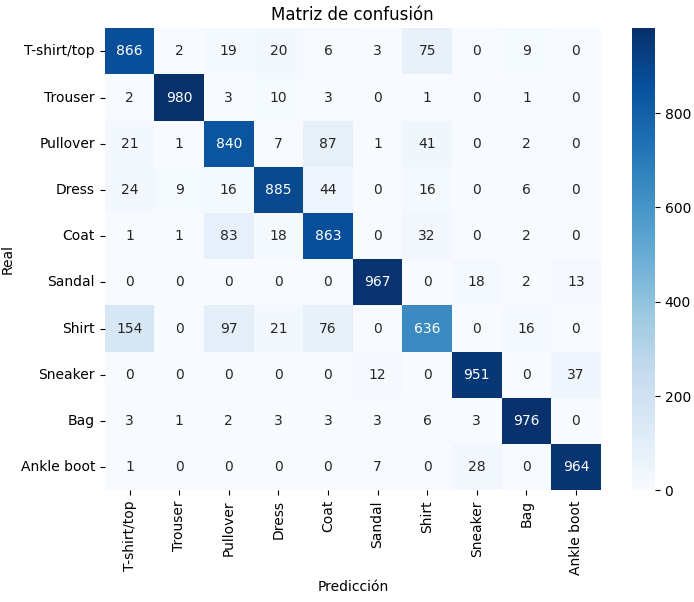
\includegraphics[width=1\textwidth]{figs/matrix_model2.png}
  \captionof{figure}{Matriz de confución modelo 2}
  \label{fig-matriz2}
\end{Figura}

\section{Conclusiones}

En este trabajo se implementó una red feed forward autoencoder para clasificar
imágenes de Fashion-MNIST. Se entrenaron tres modelos con diferentes 
hiperparámetros y se compararon los resultados obtenidos. Se observó que el 
modelo 2, que utiliza el optimizador Adam, tiene un mejor desempeño que los 
otros modelos, ya que converge más rápido y tiene una precisión más alta. Por 
otro lado, se observó que aumentar las épocas de entrenamiento no 
necesariamente mejora el desempeño de la red, ya que el modelo 3, que tiene 
el doble de épocas que el modelo 2, tiene una precisión similar. 

Por último, se analizó la matriz de confusión del modelo 2 y se observó que la red 
clasifica correctamente la mayoría de las imágenes, pero tiene problemas para 
clasificar las categorías T-shirt/top y Shirt, ya que son muy similares. Y en 
las categorías donde hay menos imágenes parecidas, la red clasifica 
correctamente la mayoría de las imágenes.

\bibliography{ref}

% Specify following sections are appendices. Use \appendix* if there
% only one appendix.

%\onecolumngrid


\end{document}
%
% ****** End of file apstemplate.tex ******